Let $\mathrm{E} = (E,\#,\vdash)$ be an event structure where
$E = \s{e_1, e_2, ...,e_n}$ and $\mathcal{C}$ be a subset of
$\mathcal{P}(E)$, we define the causal model
$\mathfrak{M}(\mathrm{E},\mathcal{C}) = (\mathcal{S},\mathscr{F},\mathcal{E})$
where
$\mathcal{S} = (\mathcal{U},\mathcal{V},\mathcal{R})$.
We define $\mathcal{U}$ to be empty and $\mathcal{V}$ as follows:
\begin{align*}
    \mathcal{V} = & \s{C_{e_i,e_j} |  1 \leq i < j \leq n.
    e_i \in E \amp e_j \in E}                                \\
                  & \cup \s{EN_{s,e} | s \in \mathcal{P}(E),
    e \in E. e \not \in s }                                  \\
                  & \cup \s{M_{s,e} | s \in \mathcal{P}(E),
        e \in E. e \not \in s } \cup \s{ES,IC}
\end{align*}
Let $\mathcal{R}(ES) = \mathbb{E}$ where $\mathbb{E}$ is the set of all
triples of the form $(E',\#',\vdash')$ where $\#' \subseteq E \times E$
and $\vdash' \subseteq \mathcal{P}(E') \times E'$ and we define all other
variables to be boolean.
For each variable $x \in \mathcal{V}$ we define $\vec V_x$ as a vector
of all variables in $\mathcal{V}$ excluding $x$.
For $x,y \in \mathcal{P}(E)$ we say $x$ is covered by $y$ written $ x \prec y$ iff:
\begin{align*}
    x \subseteq y \amp x \neq y \amp
    (\forall z. x \subseteq z \subseteq y \Rightarrow x = z
    \text{ or } y = z)
\end{align*}
We define the functions in $\mathscr{F}$ as follows:
$$
    \f{C_{e,e'}} = \begin{cases}
        true  & \text{ if } e \# e' \amp e' \# e \\
        false & \text{ otherwise }
    \end{cases}
$$
$$
    \f{M_{s,e}} = \begin{cases}
        Min(s,e) \wedge Con(s) & \text{ if } s \vdash_{min} e \\
        false                  & \text{ otherwise }
    \end{cases}
$$
\begin{align*}
    \f{EN_{s,e}} & =
    \left(
    M_{s,e} \vee
    \left(
    \bigvee_{s'\prec s}EN_{s',e}
    \right)
    \right)
    \bigwedge
    Con(s)
\end{align*}
Where we have:
\begin{align*}
    Con(s)   & =   \left(
    \bigwedge_{ 1\leq j<j' \leq n \wedge e_j,e_{j'} \in s}
    \neg C_{e_j,e_{j'}}
    \right)               \\
    Min(s,e) & = \left(
    \bigwedge_{s'. (s' \subset s \vee s \subset s')
        \wedge e \notin s'}
    \neg M(k',i)
    \right)
\end{align*}
Additionally, we define:
\begin{align*}
    \f{ES} = (E,\#',\vdash')
\end{align*}
where we have:
\begin{align*}
    \forall e,e' \in E. e \#' e' \wedge e' \#' e
     & \iff C_{e,e'} = \T \\
    \forall s \in \mathcal{P}(E), e \in E.  s \vdash' e
     & \iff EN_{s,e} = \T
\end{align*}
Intuitively, the value of $ES$ represents the event structure induced
regarding the current setting of variables.
We define the function of $IC$ to determine whether $ES$
contains any element of $\mathcal{C}$:
\begin{align*}
    \f{IC} = \bigvee_{c \in \mathcal{C}}c \in \mathcal{F}(ES)
\end{align*}
Note that since we have defined $\mathcal{U}$ to be empty and
\textcolor{red}{the model is recursive}, the values of all variables in
$\mathcal{V}$ can be uniquely determined in the model.

We define $\mathcal{E}$ to be the set of all allowable
settings of the endogenous variables such as $\vec v'$
for which if $M \vDash \vec V = \vec v' \wedge ES = \mathrm{E}'$
then $\mathrm{E}'$ is an event structure.

\subsection{Actual Cause of Property Violation}
\begin{definition}
    Given a set of events $E$, we define a safety property $P$ to be a
    subset of $\mathcal{P}(E)$.
\end{definition}
\begin{definition}
    Given an event structure $\mathrm{E}$ we say it is safe regarding the 
    property $P$ if $\mathcal{F}(\mathrm{E}) \subseteq P$.
\end{definition}

Let $E$ be set of events and $\mathrm{E} = (E,\#,\vdash)$ be an event structure.
Let $P \subseteq \mathcal{P}(E)$ be a safety property that is violated in 
$\mathrm{E}$.
The property is violated if any $c \in \mathcal{P}(E) - P$ be a configuration
of $\mathrm{E}$. 
Thus to find the actual cause of the property violation we need to find 
the actual cause of 
$\bigvee_{c \in \mathcal{P}(E) - P}c \in \mathcal{F}(\mathrm{E})$.
\begin{definition}
    Given a set of events $E$, let $P$ be a safety property on $E$ and 
    $\mathrm{E} = (E,\#,\vdash)$ be an event structure where $P$ is violated.
    If $\mathcal{M} = \mathfrak{M}(\mathrm{E}, P - \mathcal{P}(E))$
    be a causal model then $\vec X = \vec x$ is
    an actual cause of the violation of $P$ in $\mathrm{E}$ if the
    following three conditions hold:
    \begin{itemize}
        \item  \textbf{AC1.} $M\models \vec X = \vec x
                  \wedge \bigvee_{c \in \mathcal{P}(E) - P}c \in \mathcal{F}(\mathrm{E})$.
        \item  \textbf{AC2. }There exists a partition $(\vec Z, \vec W)$ of $\mathcal{V}$ with $\vec X \subseteq \vec Z$ and some setting $(\vec x',\vec w')$ of the variables in $(\vec X,\vec W)$ such that if $(M,\vec u)\models \vec Z = z^*$ for all $Z\in \vec Z$, then both of the following conditions hold:

              (a) $M \models[\vec X \leftarrow \vec x', \vec W \leftarrow \vec w']
                  IC = \F
                  \wedge \vec V = \vec v
                  \wedge  \vec v \in \mathcal{E}$.

              (b) $M \models[\vec X\leftarrow \vec x, \vec W' \leftarrow \vec w', \vec Z'\leftarrow \vec z^*]
                  IC = \T
                  \wedge \vec V = \vec v
                  \wedge \vec v \in \mathcal{E}$
              for all subsets $\vec W'$ of $\vec W$ and all subsets $Z'$ of $\vec Z$.

        \item  \textbf{AC3.} $\vec X$ is minimal; no subset of $\vec X$ satisfies conditions $AC1$ and $AC2$.
    \end{itemize}
    Where $\vec v$ is the value of endogenous variables.
\end{definition}
\pagebreak


\subsection{Examples}
\newcommand{\ra}    { \rightarrow }
\newcommand{\sem}[1]{ \llbracket #1 \rrbracket }

\begin{exmp}
\begin{figure}
\centering
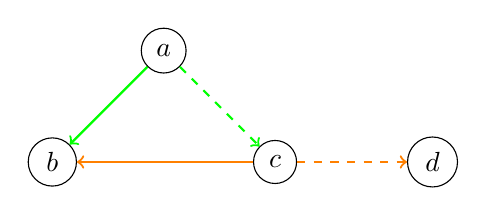
\begin{tikzpicture} [
    node distance={20mm},
    main/.style = {draw, circle},
    s/.style = {->,thick},
    d/.style = {->,thick,dashed}
  ]
  \node[main] (b) {$b$};
  \node[main] (a) [above right of=b] {$a$};
  \node[main] (c) [below right of=a] {$c$};
  \node[main] (d) [right of=c] {$d$};
  \draw[thick,green,->] (a) -- (b);
  \draw[thick,green,->,dashed] (a) -- (c);
  \draw[thick,orange,->] (c) -- (b);
  \draw[thick,orange,->,dashed] (c) -- (d);
\end{tikzpicture}
\caption{Failure of blacklist property}
\label{fig:blacklist}
\end{figure}

Blacklisted nodes are nodes in the network that must not
be reachable.
Let's assume the network in Fig. \ref{fig:blacklist} as
an example where the node $d$ is blacklisted.
For simplicity we assume that we require
$d$ not reachable only from $a$.
Consider the following DyNetKAT program for this network:
\begin{equation*}
\begin{aligned}[c]
    P   & = p!1                             \\
    Q   & = q!1                             \\
    N   & = F \oplus p?1;N_p \oplus q?1;N_q \\
    N_p & = F_p \oplus q?1;F_{pq}           \\
    N_q & = F_q \oplus p?1;F_{pq}           \\
    F   & = a\ra b \oplus c\ra b            \\
\end{aligned}
\qquad\qquad
\begin{aligned}[c]
    F_p         & = a\ra c \oplus c\ra b \oplus a\ra b \\
    F_q         & = a\ra b \oplus c\ra d               \\
    F_{pq}      & = a\ra c \oplus c\ra d \oplus a\ra d \\
    SDN         & = \delta_{\mathcal{L}} (N
    \parallel P \parallel Q)                           \\
    \mathcal{L} & = \set{p!1,p?1,q?1,q?1}                \\
\end{aligned}
\end{equation*}
We assume that there are two concurrent processes for updating
the switches $a$ and $c$.
Let we use $p$ and $q$ to denote $rcfg(p,1)$ and
$rcfg(q,1)$ respectively.
Thus, $p$ and $q$ replace the solid green and orange
paths in the network with dashed paths respectively.

Obviously, executing both $rcfg_{p,1}$ and $rcfg_{q,1}$ leads
to a state where we can forward the $\sigma_a$ to $d$.
To find the cause of error, let $\es = \sem{SDN}$ and $M$
be the causal model of $\es$, where we encode the unsafe behavior 
as:
\begin{equation*}
  \varphi = \exists X \in \conf{\es}.\;\exists e \in X.\;l(e) = a \ra d
\end{equation*}

The property above sets the value of $\varphi$ to True if $\es$ 
contains a configuration with an event labeled $a \ra d$.
In $SDN$ there are two orders of execution for $p$ and $q$; hence,
there are two events for each of these labels in $\es$ 
and thus, there are two events with the label $a \ra d$ as well.
So, let's consider events $p_1,p_2$ with label $p$,
events $q_1,q_2$ with label $q$ and events $ad_1,ad_2$ 
with label $a \ra d$ in $E$. Fig. \ref{fig:blacklist:lattice}
shows a portion of the $\conf{\es}$ lattice, which consists of configurations
which lead to events labeled with $a\ra d$.

\newcommand{\crd}[4][above]{
  \node[draw,circle,inner sep=2pt,fill,label={[#1]:#4}] at (#2,#3) {};
}

\begin{figure}
\centering
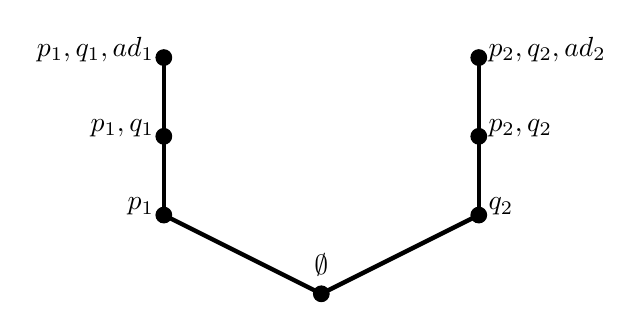
\begin{tikzpicture}
  \crd{0}{0}{$\emptyset$}
  \crd[left]{-2}{1}{$\set{p_1}$}
  \crd[left]{-2}{2}{$\set{p_1,q_1}$}
  \crd[left]{-2}{3}{$\set{p_1,q_1,ad_1}$}
  \crd[right]{2}{1}{$\set{q_2}$}
  \crd[right]{2}{2}{$\set{p_2,q_2}$}
  \crd[right]{2}{3}{$\set{p_2,q_2,ad_2}$}
  \draw [ultra thick] (-2,1) -- (-2,2);
  \draw [ultra thick] (-2,2) -- (-2,3);
  \draw [ultra thick] (0,0) -- (2,1);
  \draw [ultra thick] (0,0) -- (-2,1);
  \draw [ultra thick] (2,1) -- (2,2);
  \draw [ultra thick] (2,1) -- (2,3);
\end{tikzpicture}
\caption{Configurations lattice for the blacklist network}
\label{fig:blacklist:lattice}
\end{figure}


\usetikzlibrary{shapes.geometric}


\begin{figure}
\centering
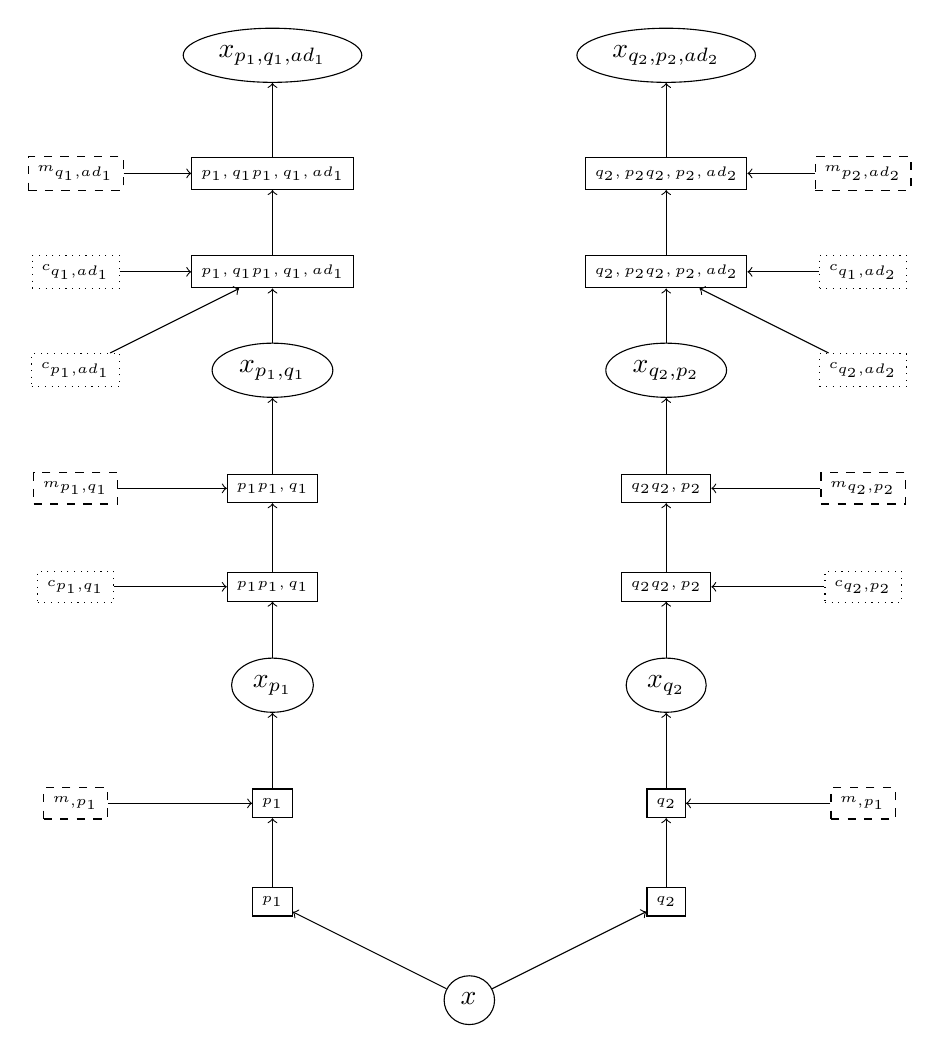
\begin{tikzpicture}
  \tikzset{
    _x/.style={ellipse,draw},
    r/.style={rectangle,draw,font=\tiny},
    m/.style={rectangle,draw,dashed,font=\tiny},
    c/.style={rectangle,draw,dotted,font=\tiny},
  }

  \node[_x] (x-null)    at (0,0)  {$x_{\varnothing}$};
  \node[_x] (x-p1)      at (-2.5,4) {$x_{ \set{p_1} }$};
  \node[_x] (x-p1q1)    at (-2.5,8) {$x_{ \set{p_1,q_1} }$};
  \node[_x] (x-p1q1ad1) at (-2.5,12) {$x_{ \set{p_1,q_1,ad_1} }$};
  \node[_x] (x-q2)      at (2.5,4)  {$x_{ \set{q_2} }$};
  \node[_x] (x-q2p2)    at (2.5,8)  {$x_{ \set{q_2,p_2} }$};
  \node[_x] (x-q2p2ad2) at (2.5,12)  {$x_{ \set{q_2,p_2,ad_2} }$};

  \node[r] (rc-null-p1)      at (-2.5,1.25) {$\rc{\varnothing}{ \set{p_1} }$};
  \node[r] (rm-null-p1)      at (-2.5,2.5) {$\rM{\varnothing}{ \set{p_1} }$};
  \node[r] (rc-p1-p1q1)      at (-2.5,5.25) {$\rc{ \set{p_1} }{ \set{p_1,q_1} }$};
  \node[r] (rm-p1-p1q1)      at (-2.5,6.5) {$\rM{ \set{p_1} }{ \set{p_1,q_1} }$};
  \node[r] (rc-p1q1-p1q1ad1) at (-2.5,9.25) {$\rc{ \set{p_1,q_1} }{ \set{p_1,q_1,ad_1} }$};
  \node[r] (rm-p1q1-p1q1ad1) at (-2.5,10.5) {$\rM{ \set{p_1,q_1} }{ \set{p_1,q_1,ad_1} }$};

  \node[r] (rc-null-q2)      at (2.5,1.25) {$\rc{\varnothing}{ \set{q_2} }$};
  \node[r] (rm-null-q2)      at (2.5,2.5) {$\rM{\varnothing}{ \set{q_2} }$};
  \node[r] (rc-q2-q2p2)      at (2.5,5.25) {$\rc{ \set{q_2} }{ \set{q_2,p_2} }$};
  \node[r] (rm-q2-q2p2)      at (2.5,6.5) {$\rM{ \set{q_2} }{ \set{q_2,p_2} }$};
  \node[r] (rc-q2p2-q2p2ad2) at (2.5,9.25) {$\rc{ \set{q_2,p_2} }{ \set{q_2,p_2,ad_2} }$};
  \node[r] (rm-q2p2-q2p2ad2) at (2.5,10.5) {$\rM{ \set{q_2,p_2} }{ \set{q_2,p_2,ad_2} }$};

  \node[m] (m-null-p1)       at (-5,2.5)  {$m_{\varnothing, p_1 }$};
  \node[m] (m-p1-q1)         at (-5,6.5)  {$m_{\set{p_1}, q_1 }$};
  \node[m] (m-q1-ad1)        at (-5,10.5) {$m_{\set{q_1}, ad_1 }$};

  \node[m] (m-null-q2)       at (5,2.5)  {$m_{\varnothing, p_1 }$};
  \node[m] (m-q2-p2)         at (5,6.5)  {$m_{\set{q_2}, p_2 }$};
  \node[m] (m-p2-ad2)        at (5,10.5) {$m_{\set{p_2}, ad_2 }$};

  \node[c] (c-p1-q1)         at (-5,5.25) {$c_{ p_1,q_1 }$};
  \node[c] (c-p1-ad1)        at (-5,8)    {$c_{ p_1,ad_1 }$};
  \node[c] (c-q1-ad1)        at (-5,9.25) {$c_{ q_1,ad_1 }$};

  \node[c] (c-q2-p2)         at (5,5.25) {$c_{ q_2,p_2 }$};
  \node[c] (c-q2-ad2)        at (5,8)    {$c_{ q_2,ad_2 }$};
  \node[c] (c-p2-ad2)        at (5,9.25) {$c_{ q_1,ad_2 }$};

  \draw[->] (x-null)          -- (rc-null-p1);
  \draw[->] (rc-null-p1)      -- (rm-null-p1);
  \draw[->] (rm-null-p1)      -- (x-p1);
  \draw[->] (x-p1)            -- (rc-p1-p1q1);
  \draw[->] (rc-p1-p1q1)      -- (rm-p1-p1q1);
  \draw[->] (rm-p1-p1q1)      -- (x-p1q1);
  \draw[->] (x-p1q1)          -- (rc-p1q1-p1q1ad1);
  \draw[->] (rc-p1q1-p1q1ad1) -- (rm-p1q1-p1q1ad1);
  \draw[->] (rm-p1q1-p1q1ad1) -- (x-p1q1ad1);
  
  \draw[->] (x-null)          -- (rc-null-q2);
  \draw[->] (rc-null-q2)      -- (rm-null-q2);
  \draw[->] (rm-null-q2)      -- (x-q2);
  \draw[->] (x-q2)            -- (rc-q2-q2p2);
  \draw[->] (rc-q2-q2p2)      -- (rm-q2-q2p2);
  \draw[->] (rm-q2-q2p2)      -- (x-q2p2);
  \draw[->] (x-q2p2)          -- (rc-q2p2-q2p2ad2);
  \draw[->] (rc-q2p2-q2p2ad2) -- (rm-q2p2-q2p2ad2);
  \draw[->] (rm-q2p2-q2p2ad2) -- (x-q2p2ad2);

  \draw[->] (m-null-p1)       -- (rm-null-p1);
  \draw[->] (m-p1-q1)         -- (rm-p1-p1q1);
  \draw[->] (m-q1-ad1)        -- (rm-p1q1-p1q1ad1);

  \draw[->] (m-null-q2)       -- (rm-null-q2);
  \draw[->] (m-q2-p2)         -- (rm-q2-q2p2);
  \draw[->] (m-p2-ad2)        -- (rm-q2p2-q2p2ad2);

  \draw[->] (c-p1-q1)         -- (rc-p1-p1q1);
  \draw[->] (c-p1-ad1)        -- (rc-p1q1-p1q1ad1);
  \draw[->] (c-q1-ad1)        -- (rc-p1q1-p1q1ad1);

  \draw[->] (c-q2-p2)         -- (rc-q2-q2p2);
  \draw[->] (c-q2-ad2)        -- (rc-q2p2-q2p2ad2);
  \draw[->] (c-p2-ad2)        -- (rc-q2p2-q2p2ad2);
\end{tikzpicture}
\caption{Causal graph for the blacklist network}
\label{fig:blacklist:causal-graph}
\end{figure}


The causal graph for this event structure is presented in Fig. \ref{fig:blacklist:causal-graph}.
We claim that $p_1 \cancel{\#} q_1$ is a cause of $\varphi$. To check, we only need to see
if there is a path from $c_{p_1,q_1}$ to either $x_{p_1,q_1,ad_1}$ or $x_{q_2,p_2,ad_2}$.
In this case, there is such a path; so the causality claim holds.
$q_2 \cancel{\#} p_2$ is also a cause of $\varphi$, due to symmetry.
\end{exmp}

\subsection{Causality in DyNetKAT}
We describe how to use causality for a given DyNetKAT expression.

\begin{definition}
    Given sets of events $E_0$ and $E_1$ let
    $E = \s{(0,e)|e \in E_0} \cup \s{(1,e)|e \in E_1}$.
    We define injections $\iota_k: E_k \rightarrow E$, given by
    $\iota_k(e) = (k,e)$, for $k = 0,1$.
\end{definition}

\begin{definition}
    Given sets of events $E_0$ and $E_1$ let their product $E$ be:
    \begin{align*}
        E_0 \times_* E_1 = \s{(e_0,*)|e_0 \in E_0} \cup \s{(*,e_1)|e_1 \in E_1}
        \cup \s{(e_0,e_1)|e_0 \in E_0 \wedge e_1 \in E_1}
    \end{align*}
    We define projections $\pi_i: E \rightarrow_* E_i$, given by
    $\pi_i(e_0,e_1) = e_i$, for $i=0,1$.
\end{definition}

\begin{definition}
    Let $\mathrm{E} = (E,\#,\vdash,L,l)$ be a labeled event structure and
    $M$ be its causal model with the set of variables:
    \begin{align*}
        \mathcal{V} = & \s{C_{e_i,e_j} |  1 \leq i < j \leq n.
        e_i \in E \amp e_j \in E}                                \\
                      & \cup \s{EN_{s,e} | s \in \mathcal{P}(E),
            e \in E. e \not \in s }
    \end{align*}
    Let $\alpha$ be a label and $\mathrm{E'} = \alpha \mathrm{E}$.
    We define $M' = \alpha M$ to be a causal model where:
    \begin{align*}
        \mathcal{V'} = & \s{C'_{e_i,e_j} |  1 \leq i < j \leq n.
        e_i \in E' \amp e_j \in E'}                                 \\
                       & \cup \s{EN'_{s,e} | s \in \mathcal{P}(E'),
        e \in E'. e \not \in s }                                    \\
                       & \cup \mathcal{V}
    \end{align*}
    Next, we define functions of $M'$ as follows:
    $$
        \f{C'_{e,e'}} = \begin{cases}
            \T       & \text{ if } e = \iota_0(\alpha) \vee e' = \iota_0(\alpha) \\
            C_{e,e'} & \text{ otherwise }
        \end{cases}
    $$

    $$
        \f{EN'_{s,e}} = \begin{cases}
            Con(s)                  & \text{ if } e = \iota_0(\alpha)             \\
            EN_{s',e} \wedge Con(s) & \text{ if } s = s' \cup \s{\iota_0(\alpha)} \\
            \F                      & \text{ otherwise }
        \end{cases}
    $$
\end{definition}

\begin{definition}
    Let $\mathrm{E}_0 = (E_0,\#_0,\vdash_0,L_0,l_0)$ and
    $\mathrm{E}_1 = (E_1,\#_1,\vdash_1,L_1,l_1)$ be labeled event structures
    and $M_0,M_1$ be their causal models.
    Let $(E',\#',\vdash',L',l') = \mathrm{E_0} + \mathrm{E_1}$.
    We define $M' = M_0 + M_1$ to be a causal model where we have:
    \begin{align*}
        \mathcal{V}_0 = & \s{C_{e_i,e_j}^0 |  1 \leq i < j \leq n.
        e_i \in E_0 \amp e_j \in E_0}                                 \\
                        & \cup \s{EN_{s,e}^0 | s \in \mathcal{P}(E_0)
        e \in E_0. e \not \in s }                                     \\
        \mathcal{V}_1 = & \s{C_{e_i,e_j}^1 |  1 \leq i < j \leq n.
        e_i \in E_1 \amp e_j \in E_1}                                 \\
                        & \cup \s{EN_{s,e}^1 | s \in \mathcal{P}(E_1)
        e \in E_1. e \not \in s }                                     \\
        \mathcal{V} =   & \s{C_{e_i,e_j} |  1 \leq i < j \leq n.
        e_i \in E' \amp e_j \in E'}                                   \\
                        & \cup \s{EN_{s,e} | s \in \mathcal{P}(E'),
        e \in E'. e \not \in s }                                      \\
                        & \cup \mathcal{V}_0 \cup \mathcal{V}_1
    \end{align*}
    We define the functions of $M'$ as follows:
    $$
        \f{C_{e,e'}} = \begin{cases}
            \T         & \text{ if } \exists e_0 \in E_0,e_1 \in E_1.
            (e = \iota_0(e_0) \wedge e' = \iota_1(e_1))
            \vee (e' = \iota_0(e_0) \wedge e = \iota_1(e_1))                    \\
            C^0_{e,e'} & \text{ if } \exists e_0,e_0' \in E_0. e = \iota_0(e_0)
            \wedge e' = \iota_0(e_0')                                           \\
            C^1_{e,e'} & \text{ if } \exists e_1,e_1' \in E_1. e = \iota_1(e_1)
            \wedge e' = \iota_1(e_1')
        \end{cases}
    $$
    $$
        \f{EN_{s,e}} = \begin{cases}
            Con(s) \wedge EN^0_{s_0,e_0} & \text{ if }
            \exists s_0 \in Con_0,e_0 \in E_0. s = \iota_0(s_0)
            \wedge e = \iota_0(e_0)                           \\
            Con(s) \wedge EN^1_{s_1,e_1} & \text{ if }
            \exists s_1 \in Con_1,e_1 \in E_1. s = \iota_1(s_1)
            \wedge e = \iota_1(e_1)                           \\
            \F                           & \text{ otherwise }
        \end{cases}
    $$
\end{definition}

\begin{definition}
    Let $\mathrm{E}_0 = (E_0,\#_0,\vdash_0,L_0,l_0)$ and
    $\mathrm{E}_1 = (E_1,\#_1,\vdash_1,L_1,l_1)$ be event structures and
    $M_0,M_1$ be their causal models.
    Let $(E',\#',\vdash',L',l') = E_0 \times E_1$.
    We define $M' = M_0 \times M_1$ to be a causal model where we have:
    \begin{align*}
        \mathcal{V}_0 = & \s{C_{e_i,e_j}^0 |  1 \leq i < j \leq n.
        e_i \in E_0 \amp e_j \in E_0}                                 \\
                        & \cup \s{EN_{s,e}^0 | s \in \mathcal{P}(E_0)
        e \in E_0. e \not \in s }                                     \\
        \mathcal{V}_1 = & \s{C_{e_i,e_j}^1 |  1 \leq i < j \leq n.
        e_i \in E_1 \amp e_j \in E_1}                                 \\
                        & \cup \s{EN_{s,e}^1 | s \in \mathcal{P}(E_1)
        e \in E_1. e \not \in s }                                     \\
        \mathcal{V} =   & \s{C_{e_i,e_j} |  1 \leq i < j \leq n.
        e_i \in E' \amp e_j \in E'}                                   \\
                        & \cup \s{EN_{s,e} | s \in \mathcal{P}(E'),
        e \in E'. e \not \in s }                                      \\
                        & \cup \mathcal{V}_0 \cup \mathcal{V}_1
    \end{align*}
    We define the functions of $M'$ as follows:
    $$
        \f{C_{e,e'}} = \begin{cases}
            \T & \text{ if } \pi_0(e) = \pi_0(e') \vee \pi_1(e) = \pi_1(e') \\
            C^0(\pi_0(e),\pi_0(e')) \vee  C^1(\pi_1(e),\pi_1(e'))
               & \text { if } \pi_0(e) \neq * \wedge \pi_1(e) \neq *        \\
            C^0(\pi_0(e),\pi_0(e'))
               & \text { if } \pi_1(e) = *                                  \\
            C^1(\pi_1(e),\pi_1(e'))
               & \text { if } \pi_0(e) = *                                  \\
        \end{cases}
    $$
    $$
        \f{EN_{s,e}} = \begin{cases}
            EN^0(\pi_0(s),\pi_0(e)) \wedge EN^1(\pi_1(s),\pi_1(e))
                                    & \text{ if } \pi_0(e) \neq * \wedge \pi_1(e) \neq * \\
            EN^0(\pi_0(s),\pi_0(e)) & \text{ if } \pi_1(e) = *                           \\
            EN^1(\pi_1(s),\pi_1(e)) & \text{ if } \pi_0(e) = *                           \\
        \end{cases}
    $$
\end{definition}
\begin{definition}
    Let $\mathrm{E} = (E,\#,\vdash,L,l)$ be an event structure and $M$ its
    causal model.
    For each variable $v \in \mathcal{V}$ we define a function $l(v)$ which
    returns the set of labels of this variable regarding the $l$ as follows:
    $$
        l(v) = \begin{cases}
            \s{l(e),l(e')}                     & \text{ if } \exists e,e' \in E. v = C_{e,e'} \\
            \s{l(e')| e' \in s } \cup \s{l(e)} & \text{ if }
            \exists s \subseteq E, e \in E. v = EN_{s,e}
        \end{cases}
    $$
\end{definition}

\begin{definition}
    Let $\mathrm{E} = (E,\#,\vdash,L,l)$ be an event structure and $M$ its
    causal model.
    Given a set of labels $\Lambda$, we define $M' = M\lceil \Lambda$ to be
    a causal model where we have removed any variable such as
    $x \in \mathcal{V}$ and its functions where $l(v) \not \subseteq \Lambda$.
\end{definition}

\begin{example}
    Consider the following network where we want to check a blacklist
    property, i.e. no packets arrive at $c$:
    \begin{center}
        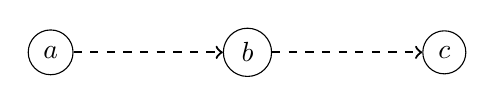
\begin{tikzpicture}[node distance={25mm},
                main/.style = {draw, circle},
                d/.style = {->,thick,dashed} ]
            \node[main] (a) {$a$};
            \node[main] (b) [right of=a] {$b$};
            \node[main] (c) [right of=b] {$c$};
            \draw[d] (a) -- (b);
            \draw[d] (b) -- (c);
        \end{tikzpicture}
    \end{center}
    We define this network using the following DyNetKAT term:
    \begin{align*}
        S_{xy}  & = sw = x \cdot sw \la y            \\
        P       & = u!S_{ab}                         \\
        Q       & = u!S_{bc}                         \\
        N_{x,y} & = (S_x+S_y)^* \oplus u?x';N_{x',y}
        \oplus u?y';N_{x,y'}                         \\
        SDN     & = N_{0,0} \parallel P \parallel Q
    \end{align*}
    We may rewrite the terms as follows:
    \begin{align*}
        N_{0,0}   & = u?S_{ab};N_{ab,0} \oplus u?S_{bc};N_{0,bc} \\
        N_{ab,0}  & = S_{ab}^* \oplus u?S_{bc};N_{ab,bc}         \\
        N_{0,bc}  & = S_{bc}^* \oplus u?S_{ab};N_{ab,cd}         \\
        N_{ab,bc} & = (S_{ab}+S_{bc})^*
    \end{align*}
    We consider this network under the situation that a single packet
    arrived at $a$.
    Thus we assume that a single packet $\sigma$ is arrived where
    $\sigma(sw) = a$.
    Under this condition, we can replace the NetKAT terms with
    packet forwarding actions of the form $(\sigma, \sigma')$.
    We use $xy$ to denote an action of the form $(\sigma,\sigma')$
    where $\sigma(sw) = x$ and $\sigma'(sw) = y$.
    For a DyNetKAT term $T$, we use $T^a$ to denote the term where
    we have replaced all NetKAT policies with packet forwarding actions.
    Given a packet $\sigma$ where $\sigma(l) = a$ we can replace NetKAT
    Furthermore, we rename actions
    $u?S_{ab},u!S_{ab},u?S_{bc},u!S_{bc}$ to $u_a,u_a',u_b,u_b'$,
    so we can derive the following terms:
    Thus we have:
    \begin{align*}
        SDN^a       & = \delta_{\mathcal{L}}(N^a_{0,0}
        \parallel P \parallel Q)                         \\
        P^a         & = u_a'                               \\
        Q^a         & = u_b'                               \\
        N^a_{0,0}   & = u_a;N^a_{ab,0} \oplus u_b;N^a_{0,bc} \\
        N^a_{ab,0}  & = ab \oplus u_b;N^a_{ab,bc}          \\
        N^a_{0,bc}  & = u_a;N^a_{ab,bc}                    \\
        N^a_{ab,bc} & = ab \oplus ac
    \end{align*}
    Let we denote $rcfg(u_a,u_a')$ and $rcfg(u_b,u_b')$ with $p$ and $q$ 
    respectively.
    Thus we can derive the following LTS for $SDN^a$:
    \begin{center}
        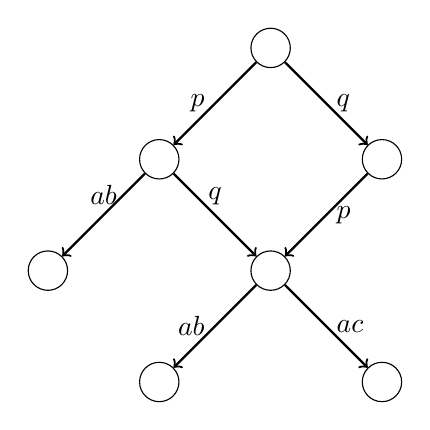
\begin{tikzpicture}[node distance={20mm},
                main/.style = {draw, circle,minimum width=5mm},
                s/.style = {->,thick}]
            \node[main] (s1) {};
            \node[main] (s2) [below left of=s1] {};
            \node[main] (s3) [below right of=s1] {};
            \node[main] (s4) [below left of=s2] {};
            \node[main] (s5) [below right of=s2] {};
            \node[main] (s6) [below left of=s5] {};
            \node[main] (s7) [below right of=s5] {};
            \draw[s] (s1) -- node[left]{$p$} (s2);
            \draw[s] (s1) -- node[right]{$q$}(s3);
            \draw[s] (s2) -- node[above]{$ab$}(s4);
            \draw[s] (s2) -- node[above]{$q$}(s5);
            \draw[s] (s3) -- node[right]{$p$}(s5);
            \draw[s] (s5) -- node[left]{$ab$}(s6);
            \draw[s] (s5) -- node[right]{$ac$}(s7);
        \end{tikzpicture}
    \end{center}
    Let $\mathrm{E} = (E,\#,\vdash,L,l)$ be the event structure of $SDN^a$
    where $L = \s{p,q,ab,ac}$.
    We define the blacklist property as follows:
    \begin{align*}
        P = \s{s \in \mathcal{P}| \forall e \in s. l(e) \neq ac}
    \end{align*}  
\end{example}